%; whizzy paragraph -pdf xpdf -latex ./whizzypdfptex.sh
%; whizzy-paragraph "^\\\\begin{frame}\\|\\\\emtext"
% latex beamer presentation.
% platex, latex-beamer $B$G%3%s%Q%$%k$9$k$3$H$rA[Dj!#(B 

%     Tokyo Debian Meeting resources
%     Copyright (C) 2012 Junichi Uekawa

%     This program is free software; you can redistribute it and/or modify
%     it under the terms of the GNU General Public License as published by
%     the Free Software Foundation; either version 2 of the License, or
%     (at your option) any later version.

%     This program is distributed in the hope that it will be useful,
%     but WITHOUT ANY WARRANTY; without even the implied warreanty of
%     MERCHANTABILITY or FITNESS FOR A PARTICULAR PURPOSE.  See the
%     GNU General Public License for more details.

%     You should have received a copy of the GNU General Public License
%     along with this program; if not, write to the Free Software
%     Foundation, Inc., 51 Franklin St, Fifth Floor, Boston, MA  02110-1301 USA

\documentclass[cjk,dvipdfmx,12pt]{beamer}
\usetheme{Tokyo}
\usepackage{monthlypresentation}

%  preview (shell-command (concat "evince " (replace-regexp-in-string "tex$" "pdf"(buffer-file-name)) "&")) 
%  presentation (shell-command (concat "xpdf -fullscreen " (replace-regexp-in-string "tex$" "pdf"(buffer-file-name)) "&"))
%  presentation (shell-command (concat "evince " (replace-regexp-in-string "tex$" "pdf"(buffer-file-name)) "&"))

%http://www.naney.org/diki/dk/hyperref.html
%$BF|K\8l(BEUC$B7O4D6-$N;~(B
\AtBeginDvi{\special{pdf:tounicode EUC-UCS2}}
%$B%7%U%H(BJIS$B7O4D6-$N;~(B
%\AtBeginDvi{\special{pdf:tounicode 90ms-RKSJ-UCS2}}

\newenvironment{commandlinesmall}%
{\VerbatimEnvironment
  \begin{Sbox}\begin{minipage}{1.0\hsize}\begin{fontsize}{8}{8} \begin{BVerbatim}}%
{\end{BVerbatim}\end{fontsize}\end{minipage}\end{Sbox}
  \setlength{\fboxsep}{8pt}
% start on a new paragraph

\vspace{6pt}% skip before
\fcolorbox{dancerdarkblue}{dancerlightblue}{\TheSbox}

\vspace{6pt}% skip after
}
%end of commandlinesmall

\title{$BEl5~%(%j%"(BDebian$BJY6/2q(B}
\subtitle{$BBh(B103$B2s(B 2013$BG/(B8$B7nEY(B}
\author{$B>e@n=c0l(B}
\date{2013$BG/(B8$B7n(B17$BF|(B}
\logo{\includegraphics[width=8cm]{image200607/openlogo-light.eps}}

\begin{document}

\begin{frame}
\titlepage{}
\end{frame}

\begin{frame}{$B@_1D=`Hw$K$46(NO$/$@$5$$!#(B}
$B2q>l@_1D$h$m$7$/$*$M$,$$$7$^$9!#(B
\end{frame}

\begin{frame}{Agenda}
\begin{minipage}[t]{0.45\hsize}
  \begin{itemize}
  \item $BCm0U;v9`(B
	\begin{itemize}
	 \item $B0{?)6X;_(B
	\end{itemize}
   \item $B:G6a$"$C$?(BDebian$B4XO"$N%$%Y%s%HJs9p(B
	\begin{itemize}
        \item $BBh(B102$B2s(B $BEl5~%(%j%"(BDebian$BJY6/2q(B
        \item Debconf
	\end{itemize}
 \end{itemize}
\end{minipage} 
\begin{minipage}[t]{0.45\hsize}
 \begin{itemize}
  \item Debian Trivia Quiz
  \item $B;vA02]Bj>R2p(B
 \end{itemize}
\end{minipage}
\end{frame}

\section{$B%$%Y%s%HJs9p(B}
\emtext{$B%$%Y%s%HJs9p(B}

\begin{frame}{$BBh(B102$B2s(B $BEl5~%(%j%"(BDebian$BJY6/2q(B}
\end{frame}

\begin{frame}{Debconf}
\end{frame}

\section{DWN quiz}
\emtext{DWN quiz}
\begin{frame}{Debian $B>o<1%/%$%:(B}

  Debian $B$N>o<1!"$b$A$m$sCN$C$F$^$9$h$M(B?
$BCN$i$J$$$J$s$FCQ$:$+$7$/$F!"CN$i$J$$$H$O8@$($J$$$"$s$J$3$H$d$3$s$J$3$H!"(B
$B$_$s$J$G3NG'$7$F$_$^$7$g$&!#(B

$B:#2s$N=PBjHO0O$O(B\url{debian-devel-announce@lists.debian.org},
\url{debian-devel@lists.debian.org} $B$KEj9F$5$l$?(B
$BFbMF$H(BDebian Project News$B$J$I$+$i$G$9!#(B

\end{frame}

\subsection{$BLdBj(B}
 %; whizzy-master ../debianmeetingresume201308.tex
% $B0J>e$N@_Dj$r$7$F$$$k$?$a!"$3$N%U%!%$%k$G(B M-x whizzytex $B$9$k$H!"(Bwhizzytex$B$,MxMQ$G$-$^$9!#(B
%

\santaku
{Sylvestre Ledru $B$,(B JDK $B$K$D$$$F%"%J%&%s%9$7$?$N$O(B}
{OpenJDK7$B$K$-$j$+$((B}
{JDK6$B$N:o=|(B}
{JDK8$B$X$N0\9T(B}
{A}
{java-common$B$r(BOpenJDK 7 $B$K@Z$jBX$($k$=$&$G$9$h!"$7$+$70lIt$N%"!<%-%F%/%A%c(B
$B$O(BOpenJDK 6$B$N$^$^!#(B}

\santaku
{OpenJDK$B#7$G%5%]!<%H$5$l$F$$$J$$%"!<%-%F%/%A%c$O$I$l$+(B}
{mipsel}
{amd64}
{i386}
{A}
{s390, mips, mipsel, kfreebsd, sparc$B$,%5%]!<%H$5$l$F$$$J$$$h$&$G$9!#(B}

\santaku
{Summer Of Code $B$N%3!<%G%#%M!<%7%g%s%a%s%P!<$G$J$$$N$OC/$+(B}
{David Bremner}
{Nicolas Dandrimont}
{Nobuhiro Iwamatsu}
{C}
{$BNcG/(BSummer of code $B%9%]%s%5!<$G3+H/$9$kFbMF$rD4@0$9$k%\%i%s%F%#%"$,$$$^(B
$B$9!#(B}

\santaku
{Brian Gupta$B$,(BDebian$B$N%H%l!<%I%^!<%/$H$7$F(BUSPTO$B$KDI2CEPO?$7$h$&$HDs0F$7$?$N$O2?$+(B}
{$B%m%4(B}
{Debian$B$NJ8;zNs(B}
{DD}
{A}
{`Debian' $B$OEPO?$5$l$F$$$?$,%m%4$OEPO?$5$l$F$$$J$+$C$?$N$GEPO?$9$k$3$H$K(B
$B$7$?$h$&$G$9!#(B}



\section{$B;vA02]Bj(B}
\emtext{$B;vA02]Bj(B}

{\footnotesize
 \begin{prework}{ dictoss }
  \begin{enumerate}
  \item (なし)
  \end{enumerate}
\end{prework}

\begin{prework}{ uwabami }
  \begin{enumerate}
  \item (なし)
  \end{enumerate}
\end{prework}

}

\section{openvpn}
\emtext{openvpn}

\begin{frame}{OpenVPN$B$G$d$j$?$$$3$H(B}
  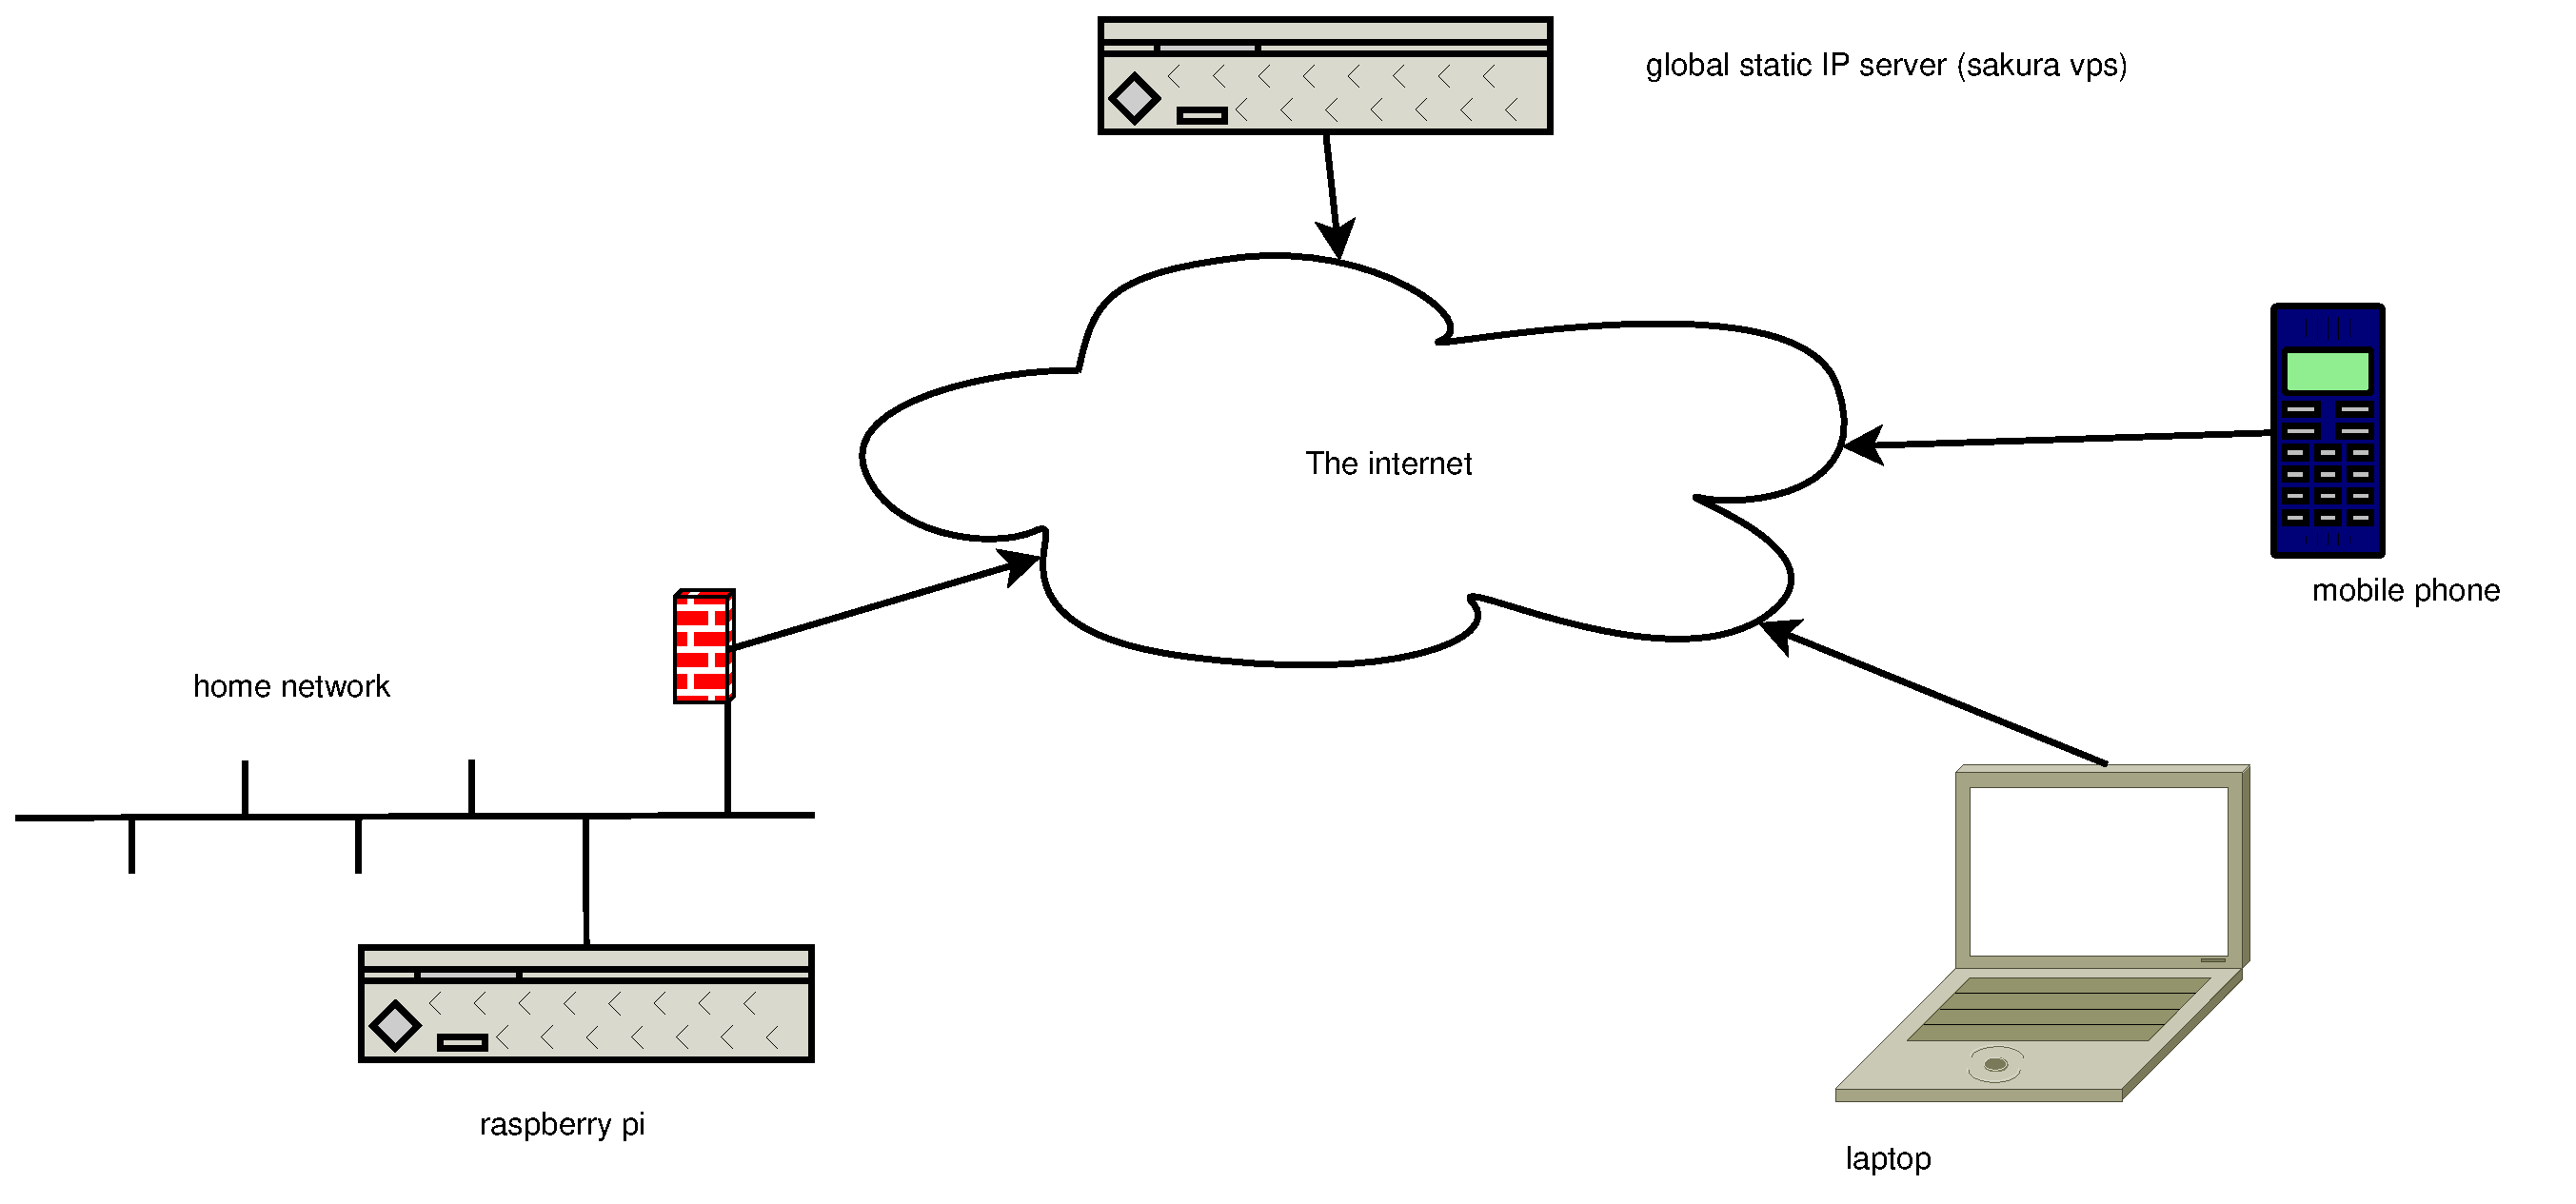
\includegraphics[width=0.9\hsize]{image201308/network.eps}
\end{frame}

\begin{frame}[containsverbatim]{$B%$%s%9%H!<%k(B}
\begin{commandline}
 # apt-get install openvpn openssl
\end{commandline}
\end{frame}

\begin{frame}[containsverbatim]{$BABDL;n83(B}
\begin{commandline}
 server$ sudo openvpn --dev tun1  \
    --ifconfig 10.1.1.1 10.1.1.2 
 client$ sudo openvpn --dev tun1  \
    --remote $B%5!<%P%[%9%HL>(B --ifconfig 10.1.1.2 10.1.11
\end{commandline}
\end{frame}

\begin{frame}[containsverbatim]{CA}
 \begin{commandline}
 # cd /etc/openvpn
 # sudo cp -R /usr/share/doc/openvpn/examples/easy-rsa/2.0/ easy-rsa/
 # cd easy-rsa/
 # vi vars
 # . ./vars
 # ./clean-all
 # ./build-ca

\end{commandline}
\end{frame}

\begin{frame}[containsverbatim]{$B%5!<%P!<80$N:n@.$H@_Dj$N:n@.(B}

\begin{commandline}
 # ./build-key-server sakura
 # ./build-dh  
\end{commandline}

\end{frame}

\begin{frame}[containsverbatim]{$B%/%i%$%"%s%H80$N:n@.(B}
\begin{commandline}
 # ./build-key client1
 # ./build-key nexus4
\end{commandline}
\end{frame}

\begin{frame}[containsverbatim]{HMAC$B80$N:n@.(B}
\begin{commandline}
 # openvpn --genkey --secret ta.key
\end{commandline}
\end{frame}

\begin{frame}[containsverbatim]{server$B@_Dj$N:n@.(B}

/etc/openvpn/server.conf $B$r:n@.$7$F(B /etc/init.d/openvpn restart

\begin{commandline}
port 1194
proto udp
dev tun
user nobody
group nogroup
tls-auth      /etc/openvpn/easy-rsa/keys/ta.key 0 # server is 0.
ca      /etc/openvpn/easy-rsa/keys/ca.crt
cert    /etc/openvpn/easy-rsa/keys/sakura.crt
key     /etc/openvpn/easy-rsa/keys/sakura.key  # keep secret
dh      /etc/openvpn/easy-rsa/keys/dh1024.pem
server 10.55.2.0 255.255.255.0  # internal tun0 connection IP
ifconfig-pool-persist ipp.txt
keepalive 10 120
comp-lzo         # Compression - must be turned on at both end
persist-key
persist-tun
status log/openvpn-status.log
verb 3  # verbose mode
client-to-client
 
\end{commandline}
\end{frame}

\begin{frame}{topology net30}

/30 $B$N(B ipv4 $B%"%I%l%9%M%C%H%o!<%/$r%/%i%$%"%s%H$4$H$K:n@.!##4(BIP$B%"%I%l%9$r(B
$B>CHq!#(B

\end{frame}

\begin{frame}{tun/tap}

\begin{tabular}{|c|p{4em}|p{8em}|p{8em}|}
\hline
 & $B%M%C%H%o!<%/%l%$%d!<(B & $B5!G=(B & $B$D$+$($k(BOS\\
\hline
tap & L2 & $B%V%j%C%8!J%V%m!<%I%-%c%9%H%Q%1%C%H$,E~C#$9$k!K(B & linux \\
tun & L3 & $B%k!<%?(B & linux, iOS, Android$B$J$I(B \\
\hline
\hline
\end{tabular}
\end{frame}

\begin{frame}[containsverbatim]{$B%/%i%$%"%s%HB&$N@_Dj(B}
\url{/etc/openvpn/*.conf}$B$K$*$$$F$*$1$P>!<j$K%M%C%H%o!<%/$KJQ99$,$"$l$P(B
 $B<B9T$5$l$k@_Dj$K$J$C$F$$$^$9!#(B

\begin{commandline}
client
dev tun
port 1194
proto udp
remote xyz.sakura.ne.jp 1194
nobind
tls-auth      ta.key 1 # client is 1.
ca ca.crt
cert android-nexus4.crt
key android-nexus4.key
remote-cert-tls server
comp-lzo
persist-key
persist-tun
verb 3
\end{commandline}
\end{frame}

\begin{frame}[containsverbatim]{Android$B$K%$%s%]!<%H(B 0}
$B%U%!%$%k$r%3%T!<(B
\begin{commandline}
$ ls -1 
android-nexus4.crt
android-nexus4.csr
android-nexus4.key
ca.crt
client.ovpn
ta.key
$ adb push . /sdcard/secure
push: ./ca.crt -> /sdcard/secure/ca.crt
push: ./android-nexus4.key -> /sdcard/secure/android-nexus4.key
push: ./ta.key -> /sdcard/secure/ta.key
push: ./android-nexus4.crt -> /sdcard/secure/android-nexus4.crt
push: ./client.ovpn -> /sdcard/secure/client.ovpn
push: ./android-nexus4.csr -> /sdcard/secure/android-nexus4.csr
\end{commandline}
\end{frame}

\begin{frame}{Android$B$K%$%s%]!<%H(B 1}

\includegraphics[height=0.9\vsize,bb=0 0 768 1280]{image201308/Screenshot_2013-08-17-16-04-31.png}

\end{frame}
\begin{frame}{Android$B$K%$%s%]!<%H(B 2}
\includegraphics[height=0.9\vsize,bb=0 0 768 1280]{image201308/Screenshot_2013-08-17-16-04-43.png}

\end{frame}
\begin{frame}{Android$B$K%$%s%]!<%H(B 3}
\includegraphics[height=0.9\vsize,bb=0 0 768 1280]{image201308/Screenshot_2013-08-17-16-04-54.png}

\end{frame}
\begin{frame}{Android$B$K%$%s%]!<%H(B 4}
\includegraphics[height=0.9\vsize,bb=0 0 768
 1280]{image201308/Screenshot_2013-08-17-16-05-07.png}
\end{frame}

\begin{frame}{Android$B$K%$%s%]!<%H(B}
$B$3$l$G%G%#%l%/%H%j:o=|$7$F$h$$$G$9!#(B
\end{frame}

\begin{frame}{$B0lJ}(Bssh$B$O(B}
 
\begin{table}[H]
 \caption{ssh $B$N5!G=$NBP1~(B}
 \begin{tabular}{|p{6em}|p{8em}|p{10em}|}
 \hline
 & ssh$B%*%W%7%g%s(B & $B5!G=(B \\
 \hline
 $B%]!<%H%U%)%o!<%G%#%s%0(B &  -L, -R & $BFCDj$N%m!<%+%k$N(BTCP$B%]!<%HHV9f$r%j%b!<%H$N%]!<%HHV(B
	 $B9f$H%^%C%T%s%0$9$k(B \\
 \hline
 $B%W%m%-%7(B & -D & SOCKS$B$KBP1~$7$F$$$k%"%W%j%1!<%7%g%s$N%W%m%-%7$rDs6!(B \\
 \hline
 VPN & -w & IP$B%l%Y%k$GAj8_$K8+$($k$h$&2>A[E*$K%M%C%H%o!<%/$r9=C[$9$k(B \\
 \hline
 \hline
 \end{tabular}
\end{table}

\end{frame}


\section{epub}
\emtext{epub}

\section{$B:#8e$N%$%Y%s%H(B}
\emtext{$B:#8e$N%$%Y%s%H(B}
\begin{frame}{$B:#8e$N%$%Y%s%H(B}
\begin{itemize}
 \item 2013$BG/(B9$B7n(B Debian$BJY6/2q(B
\end{itemize}
\end{frame}

\section{$B:#F|$N1c2q>l=j(B}
\emtext{$B:#F|$N1c2q>l=j(B}
\begin{frame}{$B:#F|$N1c2q>l=j(B}
$BL$Dj(B
\end{frame}

\end{document}

;;; Local Variables: ***
;;; outline-regexp: "\\([ 	]*\\\\\\(documentstyle\\|documentclass\\|emtext\\|section\\|begin{frame}\\)\\*?[ 	]*[[{]\\|[]+\\)" ***
;;; End: ***
